\providecommand{\main}{../main}
\documentclass[../../main.tex]{subfiles}


\begin{document}
    
    \chapter{Fast Inference of Neural Networks on FPGA}
    \chaptermark{Fast Inference of Neural Network}
    \label{sec:FPGA_NN}
    
Filed Programmable Gate Arrays (FPGA in the following) have become more and more powerful thanks to the advancement in the silicon manufacturing process, this has led to an increased adoption in a wide variety of fields from control systems to computer vision.  
Machine Learning is one of the main trends that has grown exponentially in the last few years and the aforementioned FPGA performance jump has made it possible to use them to accelerate such workloads.  
Advantages of using FPGAs over general purpose devices can be summarized in three points:  
\begin{itemize}
    \item \textbf{Parallelization}: by nature FPGAs are parallel devices, thanks to that it is possible to compute at the same time multiple operations, leading to reduced computation time. The last generation can easily outperform a server-grade GPU in inference tasks\cite{FPGA-inf}.
    \item \textbf{Efficiency}: the whole resources' pool is never required in a design, thanks to that the unused resources will not draw any power leading to a very efficient design.  
    \item \textbf{Customization}: the design must and have to be tailored to the specific task that it will have to solve, it can be made as light as possible to preserve power and area.  
\end{itemize}
    
    
\section{FPGA Architecture}
\sectionmark{FPGA Architecture}
\label{sec:FPGA_struct}

FPGAs have become more and more complex following the increased computing power that they offer, but the architecture did not change substantially. Silicon is divided in two main substructures, the computing logic and the configuration memory; the first is made of the programmable logic, arithmetic units and memory blocks, the second instead as its name suggests stores the information of the current FPGA configuration. The classification of such chips is usually made from the target environment:
\begin{itemize}
    \item \textbf{Space}: High reliability is required in such harsh environment, so configuration memories are usually made of \textit{anti-fuse}\footnote{Similar concept of fuses, but the principle is the opposite: when a high enough current flows though a permanent connection is established} or \textit{flash};
    \item \textbf{High radiation environment}: Similar to space-grade category, here the radiation tolerance is higher but the electronics can be serviced or changed;
    \item \textbf{General-purpose}: This category does not have the same strict requirements of the previous one, but offers the best computing performances, in this case only Static \acrshort{ram} (\acrshort{sram}) configuration memories are used;
\end{itemize}
        
\begin{figure*}[h]
    \begin{minipage}[c]{0.63\linewidth}
        \vspace{0pt}
        \centering
            \includegraphics[width=8.2cm]{sections/04/Images/FPGA_struct.pdf}
            \label{fig:preliminary_ssb_bkg_waveform}
    \end{minipage}%
    \hfill%
    \begin{minipage}[c]{0.37\linewidth}
        \vspace{0pt}
        \centering
            \includegraphics[width=5.8cm]{sections/04/Images/VirtexHBM.png}
            \label{fig:preliminary_ssb_bkg_integrals}
    \end{minipage}%
    \caption{On the left a schematic view of a FPGA architecture, on the right a Xilinx-AMD Virtex VU57P where on the bottom it is possible to see  the dies of the HBM memory.}
    \label{fig:FPGA_Arch}
\end{figure*}
    
\subsection{FPGA Main elements}
\label{sec:FPGA_elements}
The main blocks are:
\begin{itemize}
    \item \textbf{CLB}: \acrlong{clb}, it is the main resource for implementing general-purpose combinatorial and sequential circuits. It consists of \acrfull{lut} where a specific function or behaviour is stored, Flip-Flops (FF) that register the signal, Multiplexers (MUX) that act like a selector, Carrys for additions and mathematical operations.  
    
    \begin{minipage}{\linewidth}
        \centering
        \includegraphics[width=7.3cm]{sections/04/Images/FPGA_CLB.pdf}
        \captionof{figure}{Simplified diagram of a CLB, the output can be registered with the input clock or not.}
    \end{minipage}
    \item \textbf{BRAM}: \acrlong{bram}, configurable memory that can be used as \textit{cache} for internal computing or as \textit{buffer} to align or store temporarily the incoming data.
    \item \textbf{DSP}: \acrlong{dsp}, it is used for a wide variety of digital processing tasks. It features a pre-adder, a multiplier, a pattern detector and multiple flip-flops. The latter can be instantiated between two operations, doing so it will be easier for the design to achieve higher frequencies.  
    \begin{minipage}{\linewidth}
        \centering
        \includegraphics[width=9cm]{sections/04/Images/DSP48E2.png}
        \captionof{figure}{Diagram of a DSP block within the Ultrascale+ architecture.}
    \end{minipage}
    \item \textbf{Clocking}: Most important signals in a synchronous design are \textit{clocks} and \textit{resets}, to maintain them as clean as possible dedicated global and regional routing networks are reserved only for them.  
    \item \textbf{I/O block}: This block is used to receive and send signals to the outer world, it pack several sub-modules such as tri-state buffers, deserializers, different standard interface, ecc.
    \item \textbf{Hard IP Core}: Some functions that are often used in digital design are built directly on the FPGA's silicon die following an \acrshort{asic}-like approach. Doing so that particular function can reach higher frequency and efficiency, examples of such blocks are: hard processors (generally ARM processors), gigabit-transcievers or clock related modules (\acrshort{pll} and \acrshort{mmcm} Fig. \ref{fig:MMCM}).
    \begin{minipage}{\linewidth}
        \centering
        \includegraphics[width=9cm]{sections/04/Images/PLL.jpg}
        \captionof{figure}{Diagram of an MMCM block, used to clean the clock coming from the external world.}
        \label{fig:MMCM}
    \end{minipage}
\end{itemize}
        
\subsection{Super Logic Region (SLR) concept}
\label{sec:FPGA_SLR}
\begin{figure}[h]
    \centering
    \includegraphics[width=0.7\textwidth]{sections/04/Images/FPGA_SLRCROSS.pdf}
    \caption{SLR concept, crossing two SLR require a chain of flip-flops to avoid potential timing violations.}
    \label{fig:SLR-CROSS}
\end{figure}
        
The last generation of FPGAs are built in such a way that multiple silicon dies are stacked together with a technology called \acrfull{ssi} where different dies, homogeneous or heterogeneous\footnote{they can be based on the same die or different dies, for example SLRs and 28G transceivers}, are connected via a passive silicon interposer, in this way higher resource density is achieved. The different dies are called \acrfull{slr}. This process introduce some drawbacks in the firmware design phase, in fact signals that need to travel one or multiple SLRs, SLR crossing in the following, have a timing penalty leading to an higher latency and increased routing difficulty.  
In the design to take care of such SLR crossing, multiple flip-flops have to be instantiated\footnote{their number varies in function of the target frequency and the width of the transiting signal}, on top of that this jump can be only performed in specific regions of the chip and their number is limited. An example on how to manage an SLR crossing is given in Fig. \ref{fig:SLR-CROSS}.
        
        
        
\subsection{Timings}
\label{sec:FPGA_timings}

Synchronous digital electronics has many advantages over the asynchronous counterpart, but some design aspect must be followed. To maintain its deterministic behaviour, synchronous signals must arrive at the same clock tick, which means that the delay introduced by logic and routing must be below a certain value, if the value is too high some signals can be registered in the wrong clock cycle leading to a mismatch with the expected behaviour.
Key metric to monitor during the implementations step it's the so-called \acrfull{wns}; the latter takes into account multiple parameters, logic delay, net delay and  clock uncertainty to name a few, then it computes the difference between the maximum allowed delay and the sum of the introduced delays, if this number is positive the timings are met if not some actions must be taken.  
        
The second metric to monitor is the \acrfull{whs}, this metric is related to clock domain crossing; a signal to be correctly sampled must be stable for a given time before and after the sampling, generally  the clock rising edge. If a signal crosses two clock domains it is possible that it will be sampled in a \textit{metastable} state where its value is not predictable, to avoid this issue some module called synchronizer must be instantiated.  
        
\subsubsection{Timing closure techniques}

There are many techniques to tackle the aforementioned problem.  
Firstly, the design must be properly constrained, clocks must be declared and critical paths must be treated carefully. 

\begin{figure}[h]
    \centering
    \includegraphics[width=0.7\textwidth]{sections/04/Images/FF_piplineing.pdf}
    \caption{To achieve high frequency it is necessary to pipeline critical operations in multiple clock cycles.}
    \label{fig:FF_pipline}
\end{figure}

\textbf{Floor Planning}: high clock frequency means less time between two clock cycles and by extent signals can't travel long nets. Floor planning becomes critical, for example modules that compute input from the transceivers have to be close to them to reduce connection length. This type of directives are set via a constraint file usually in a .tcl script or a .xdc file.  

\textbf{Critical Path Analysis}: timing reports can be exploited to spot potential critical paths that cannot reach timing closure, redesigning only such signals. As shown in Fig. \ref{fig:FF_pipline}, multiple registers can be used to pipeline the computation allowing signals to travel greater distances at the price of increased latency.

\textbf{Clock Domain Crossing (CDC)}: when a signal pass through two clock domains if no countermeasures are taken, timing violations can arise. There are many solutions to this issue. The simplest one is to register multiple time the same signal and then cross the two domains, other advanced solutions can be asynchronous FIFOs, handshake signals or vendor macros.

\textbf{Synthesis and Implementation directives}: during the synthesis and implementation the tool can be instructed to try multiple iteration in the place and route phase, this can lead to timing closure at the price of increased compilation time. Not all directives can reach the desired outcome, for this reason a grid search can be used: multiple runs with different strategies can run in parallel and the best one is picked.

\textbf{Over-constraining the design}: harsher constraint can be used to force the tool to find the best implementation to meet the timing, highlighting the critical path. After that, the constraint can be lightened only in that specific path. An example of over-constraining can be increasing the clock uncertainty.
    
\sectionmark{hls4ml}
\section{\textit{hls4ml}: High Level Synthesis for Machine Learning}
\sectionmark{hls4ml}
\label{sec:FPGA_hls4ml}
%Neural Network based condition within the Phase-II GT has to meet strict constraints: latency and resource usage.
The tool-kit \textit{High Level Synthesis for Machine Learning}, or \textit{hls4ml} in short, offers an easy workflow to implement neural network modules within the FPGA programmable logic. FPGAs are generally programmed via \acrfull{hdl}, which is a language that describes an electronic circuits via gateware and flip-flops and it is not suitable for the general public of AI engineers due to its intrinsic low abstraction level. High level synthesis on the other hand leverages C++ to develop the module logic while the hardware translation is left to the FPGA vendor tool\footnote{e.g. Vivado-HLS (AMD-Xilinx) or Intel High Level Synthesis Compiler (Intel-Altera)}.  
    
\begin{figure}[h]
    \centering
    \includegraphics[width=0.8\textwidth]{sections/04/Images/hls4ml_workflow.jpg}
    \caption{Usual workflow of hls4ml tool kit, here are highlighted the three main steps: model design and train (orange), HLS conversion and tune (blue), firmware design (black).}
    \label{fig:hls4ml}
\end{figure}

\subsection{Workflow}
\label{sec:FPGA_hls4ml_workflow}

To produce the bitfile that the board requires, four steps must be followed (Fig. \ref{fig:hls4ml}):
\begin{itemize}
    \item \textbf{Training}: Usual workflow employing the preferred framework such as \textit{Tensorflow} or \textit{Pytorch}: neural network architecture definition, training and evaluation.  
    
    In this step it is possible to start part of the optimization required to fit the model in the programmable logic.
    \item \textbf{HLS conversion}: Convert the high level model produced - generally Python - into HLS code that consists of C++ plus the so-called directives that instruct the tool on how to implement a given function, for example if the computation has to be done in a pipeline fashion or fully parallel.  
    \item \textbf{Build project}: Generate the project invoking the HLS tool, at this time it is possible to define the module's physical requirements such as FPGA model and target clock frequency.  
    \item \textbf{Custom firmware}: Once the module is exported an interface must be developed to establish the data communication, this step is left to the developer; an alternative is to use the module as a co-processing kernel, in this way it works as accelerator card (PYNQ or Alveo cards from Xilinx).
    
\end{itemize}

    
\subsection{Model Optimization}
\label{sec:FPGA_opt}
Despite the fact that the current generation FPGAs is quite powerful, Neural Network models must undergo heavy optimization to reduce their resource footprint. The resulting model must have similar performances, but the main gains are in terms of latency, simpler routability and lower resource utilization. As mentioned it is possible to tackle this problem in different ways during each step:  
\begin{itemize} 
    \item \textbf{Training}:
    \begin{itemize}
        \item Quantization: Within the training procedure inputs, weights, biases and results are described as floating point numbers, which means that each of them uses a 32-bit register. As mentioned in section \ref{sec:FPGA_elements} DSPs are 27$\times$18 bit multipliers, this implies that with greater precision inputs a single multiplication will use multiple DSP blocks, to avoid this unwanted behaviour the variables are translated from floating point to fixed point representation with tunable precision. One of the new addition to the hls4ml tool is the Quantization Aware Training where during the training the ML-framework knows the variable quantization a priori producing better result than the Post Training Quantization \cite{qkeras}. The quantization employs the ap\_(u)fixed$\left<X,Y\right>$ data types, as it is shown in Fig. \ref{fig:fixedvsfloat}, $X$ carries the integer part\footnote{With or without the sign depending if it is ap\_fixed (signed) or ap\_ufixed (unsigned)} while $Y$ carries the fractional part.
        
        \begin{minipage}{\linewidth}
            \centering
            \includegraphics[width=8cm]{sections/04/Images/FPGA-data_format.pdf}
            \captionof{figure}{Example of data format used in hls4ml: single precision (float32) and fixed precision (fixed and ufixed).}
            \label{fig:fixedvsfloat}
        \end{minipage}
        
        \item Compression: Also called pruning, this optimization involves powerful tools from the Tensorflow library \cite{tfmot}. The outcome is that a fraction of weights are set to zero, which means that some connections between neurons are erased, lowering the number of operations that have to be computed alongside the related memory.  
        
    \end{itemize}
    
    \item \textbf{HLS conversion}: 
    \begin{itemize}
        \item Precision tuning: Once the training has been accomplished another step of precision tuning can be performed, looking at the distribution of the \acrshort{lsb} (fractional part) and \acrshort{msb} (integer part) it is possible to further reduce the resource impact.
        
        \item DSP reuse:  DSPs are in general the limiting factor of this kind of conversion and how they are used can be optimized to target latency or resource usage; if latency is the target the multiplications are done in parallel, otherwise the DSPs can be used in a pipeline fashion reusing the same logic splitting the operation in multiple clock cycles, Fig. \ref{fig:DSP-reuse}.
        
        \begin{minipage}{\linewidth}
            \centering
            \includegraphics[width=8.5cm]{sections/04/Images/reuse_factor.png}
            \captionof{figure}{Example of reuse of the DSP logic to save resources.}
            \label{fig:DSP-reuse}
        \end{minipage}
        
    \end{itemize}
    
     Final result have lower LUTs, DSPs adn FFs usage and generally also lower latency with respect to the unoptimized model.
    
\end{itemize}
    

\subsection{DNN vs CNN in hsl4ml}
\label{sec:hls4ml_DNNvCNN}
In this section the main hls4ml implementation differences between Dense and Convolutional layers are shown.
\begin{itemize}
    \item \textbf{Dense layer}: The dense operation, as mentioned in sec \ref{sec:DNN}, is a matrix multiplication. The hardware counterpart is a \acrfull{mac} structure, each input is multiply by its weight and the sum of all results is taken (per output basis); the max number of parallel multiplications is set by the \textit{reuse factor}, with grater values fewer parallel products are computed concurrently\cite{hls4ml-DNN}.  
    
    A large \txtit{reuse factor} translates also in a greater Initiation Interval (II) expressed in clock cycles, it means that once the first sample is fed to the module, it cannot accept any more data for the II clock cycles.  
    
    \item \textbf{Convolutional layer}: The convolution operation is made of multiple nested loops, implementing them in a similar way to GPUs is not feasible due to limitation in resources and the lack of dedicated block for matrix multiplications. To overcome this problem hls4ml stores the input tensor in BRAMs and access them when needed\cite{hls4ml-CNN}.  
    
    This intrinsically increases the II, the minimum value is the length of the flattened input tensor.  
\end{itemize}

When to choose one over the other depends on multiple factors: external constraints such as latency, initiation interval  and resource usage, how the data is packed (streamed or fully parallel) and obviously on the task that the neural net is requested to accomplish\footnote{As an example a trigger decision must be taken in hundreds of nanoseconds with an input size of tens of variables, a CNN will be highly inefficient due to the serialization of the inputs, but some workaround can be introduced}.

\subsection{Alveo hls4ml implementation}
\label{sec:FPGA_alveo}

As mentioned in sec \ref{sec:FPGA_hls4ml}, the neural network module can be implemented with custom firmware or as a co-processing kernel. The Alveo implementation is a co-processing kernel solution, this workflow does not require to produce any VHDL code, the hls4ml add-on produce a binary file that can be directly imported in one of these cards. The firmware can be easily tested with the \textit{PYNQ} infrastructure that allows a simple access to the FPGA memory banks. This procedure is still a custom firmware that requires a the complete workflow, from training to firmware building.
    
\begin{figure*}[h]
\begin{minipage}[c]{0.5\linewidth}
    \vspace{0pt}
    \centering
        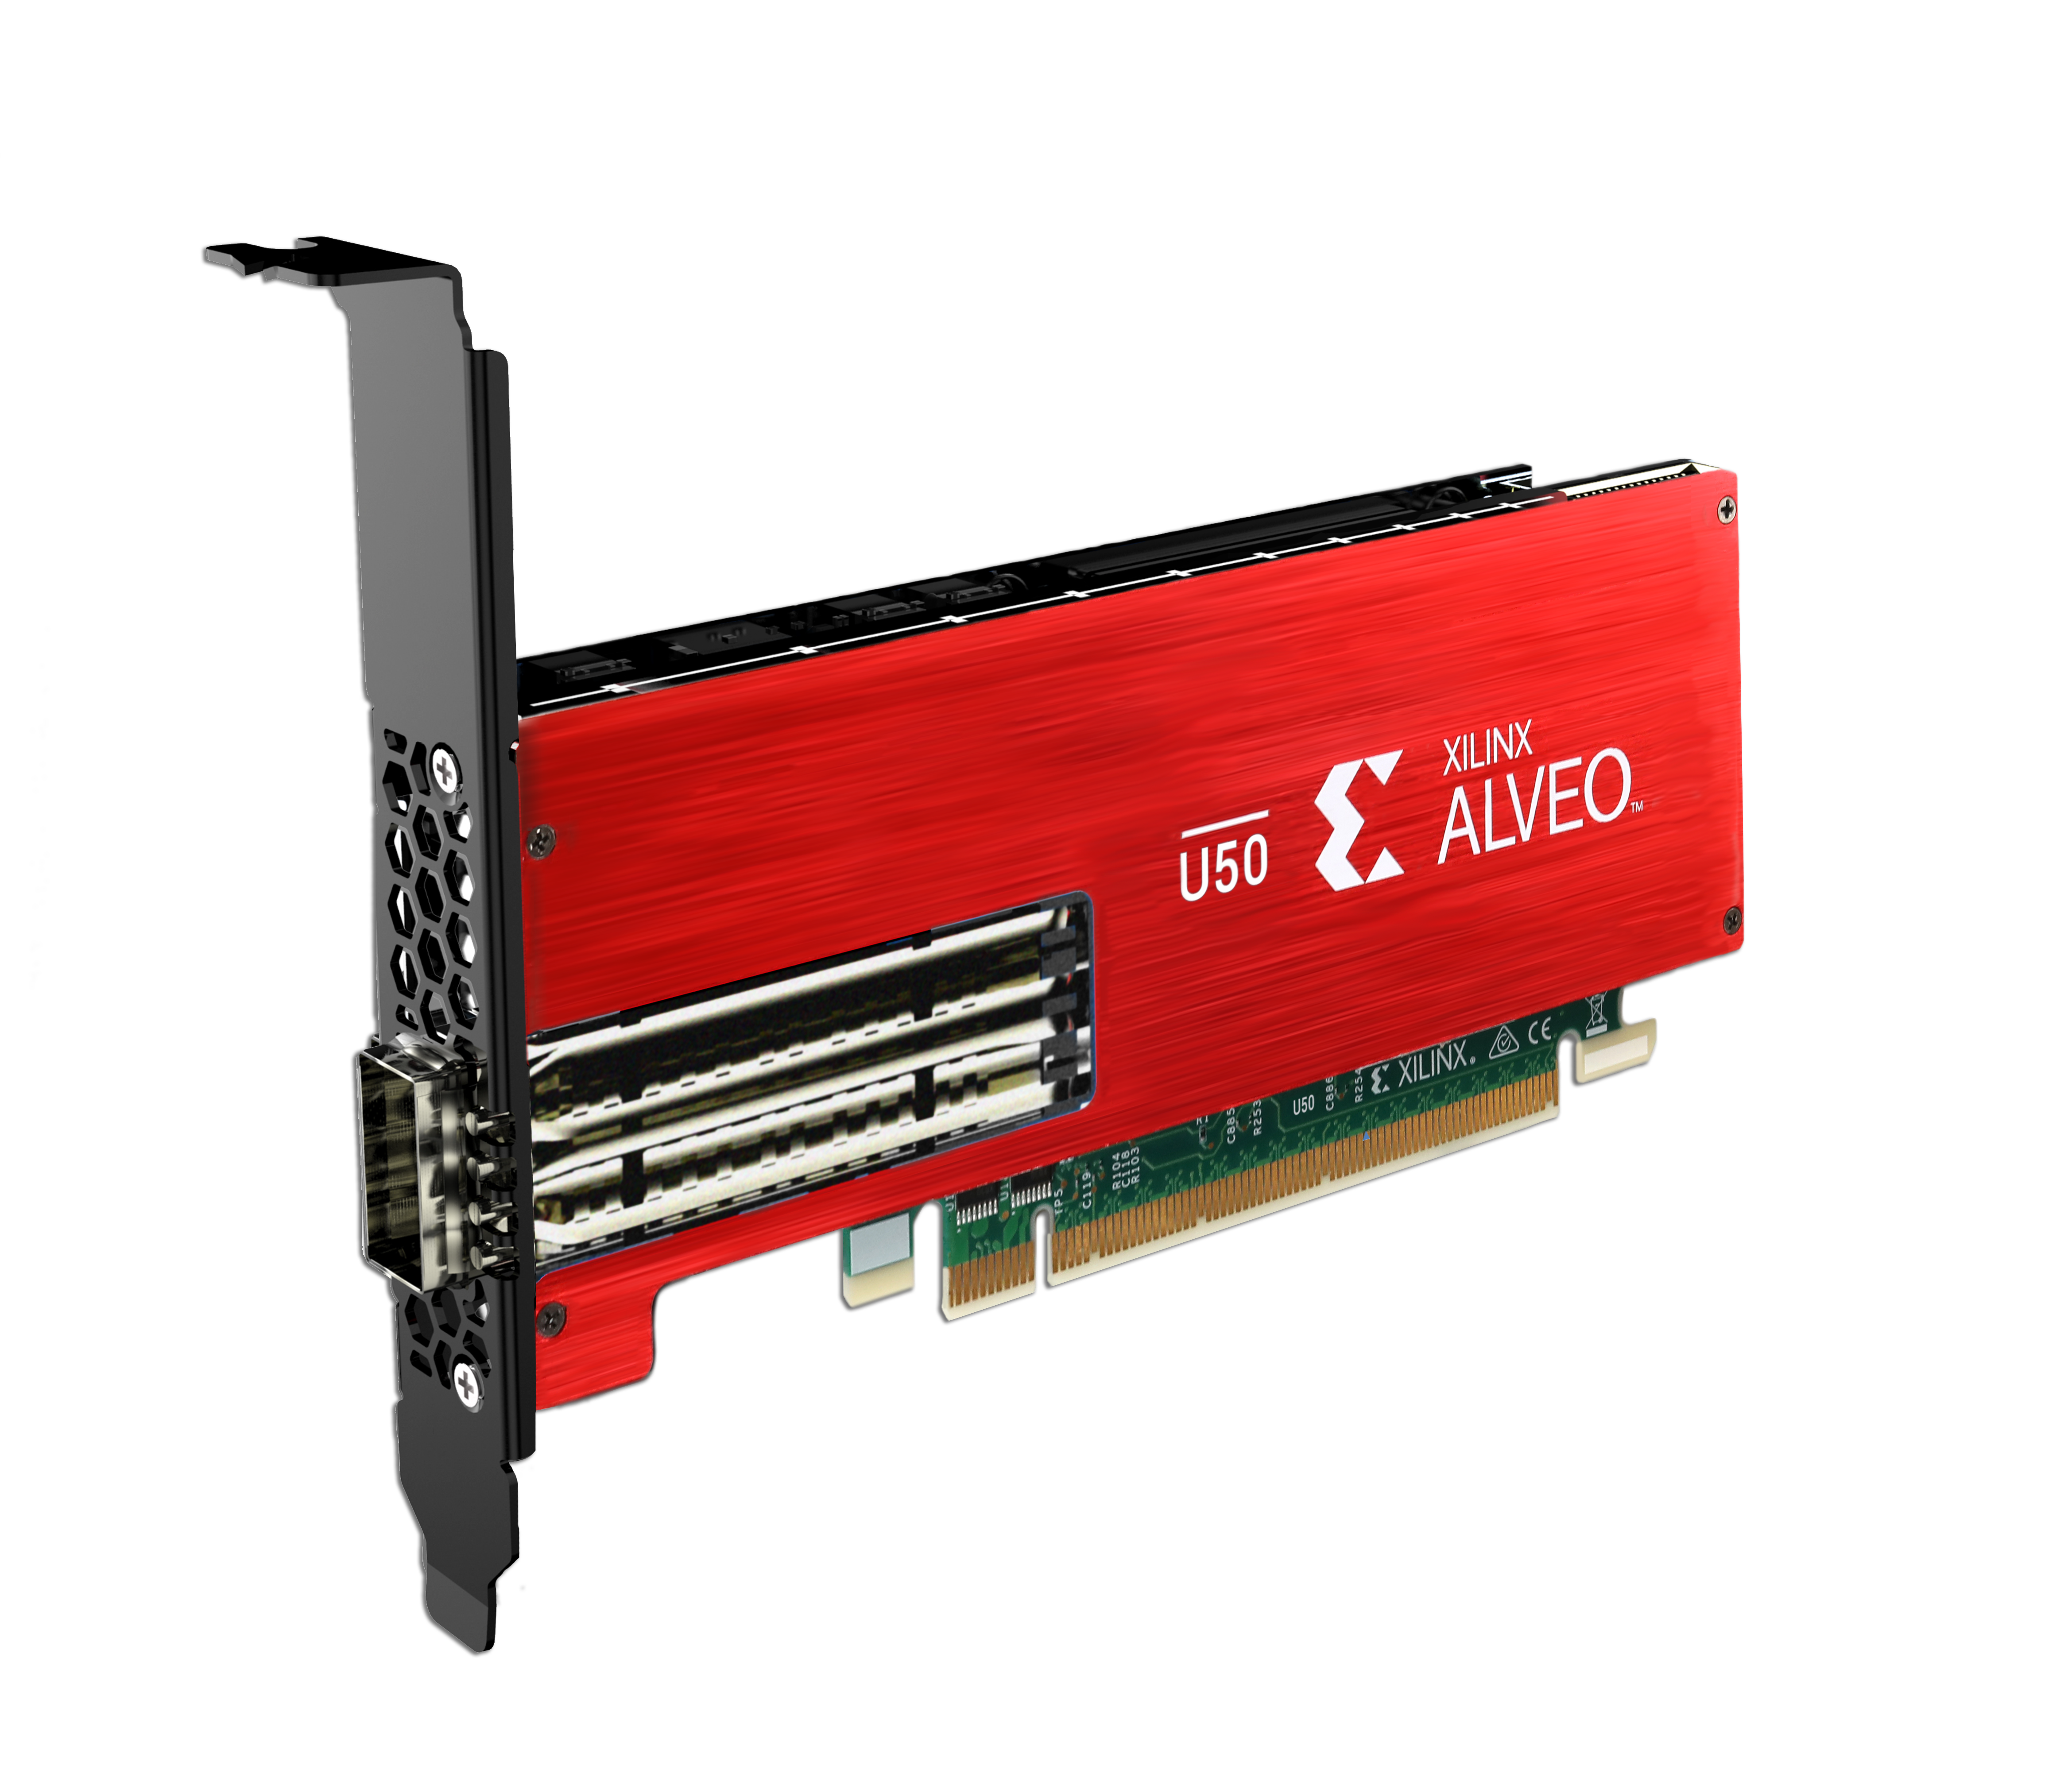
\includegraphics[width=8cm]{sections/04/Images/Alveo-U50.png}
        \label{fig:ALVEO-U50_card}
\end{minipage}%
\hfill%
\begin{minipage}[c]{0.5\linewidth}
    \vspace{0pt}
    \centering
        \includegraphics[width=8cm]{sections/04/Images/Alveo-U50-connections.pdf}
        \label{fig:ALVEO-U50_struct}
\end{minipage}%
\caption{Accelerator card Xilinx-AMD ALVEO U50, it has two SLRs: one communicates to host machine though PCIe protocol while the other communicates to the external world via a \acrshort{qsfp}}
\label{fig:ALVEO}
\end{figure*}

The Alveo U50 (Fig. \ref{fig:ALVEO}) houses an Ultrascale+ FPGA part; it feature 2 SLRs, multiple gigabit transceivers\footnote{Xilinx distinguish them in function of their performances: GTH (16.375 Gb/s), GTY (32.75 Gb/s), GTM (58 Gb/s) \cite{Xilinx-GT}} and 32 HBM banks, 256 MB each.  

The driver that allows the data transfers between host machine (linux-based) and the FPGA is the Xilinx RunTime stack (XRT) shown in Fig. \ref{fig:Alveo_XRT}. The communication from build machine (Host) and the accelerator card (Device) is made through the Xilinx RunTime stack, data are moved from the Host directly to the HBM banks or DDR memory modules via a DMA engine, then the data are accessed and the result is computed and sent back to the memory.
    
\begin{figure}[h]
    \centering
    \includegraphics[width=0.7\textwidth]{sections/04/Images/XRT-Layers.pdf}
    \caption{XRT stack.}
    \label{fig:Alveo_XRT}
\end{figure}  

This kind of implementation allows FPGAs to accelerate neural network inferences. this type of acceleration target high throughput and low latency, the same outcome cannot be reached with GPUs and CPUs\cite{ALVEO-NN}.


\end{document}